\chapter{word2vec}
\textbf{word2vec}\footnote{https://github.com/svn2github/word2vec}とは、2013年にGoogleのMikolovらが発表した、単語の分散的意味表現学習ツールである。意味表現学習の過程で解くのは、ある文脈内で共起する形態素を予測するタスクである。文脈が与えられ、次に出てくる形態素を予測するモデルを\textbf{言語モデル}という。与えられた形態素列がどれほどその言語らしいかを評価するモデルである。

言語モデルでは着目形態素の前方にある形態素のみから次に来る形態素を予測しなければならないが、意味表現獲得を目的としているため、後方の形態素も予測に使える。よって、$x_1,...,x_{i-1}$と、$x_{i+1},...,x_n$から$x_i$を予測する。

この章ではword2vecに実装されている2つの手法を紹介していく。

\section{実装アルゴリズム}
\subsection{連続単語袋詰モデル}
\textbf{連続単語袋詰モデル}(Continuous Bag-of-Words model, CBoW model)では、\textbf{文脈語}(着目形態素と共起している形態素)から着目形態素の出現確率を予測している。
\begin{figure}[h]
  \centering
  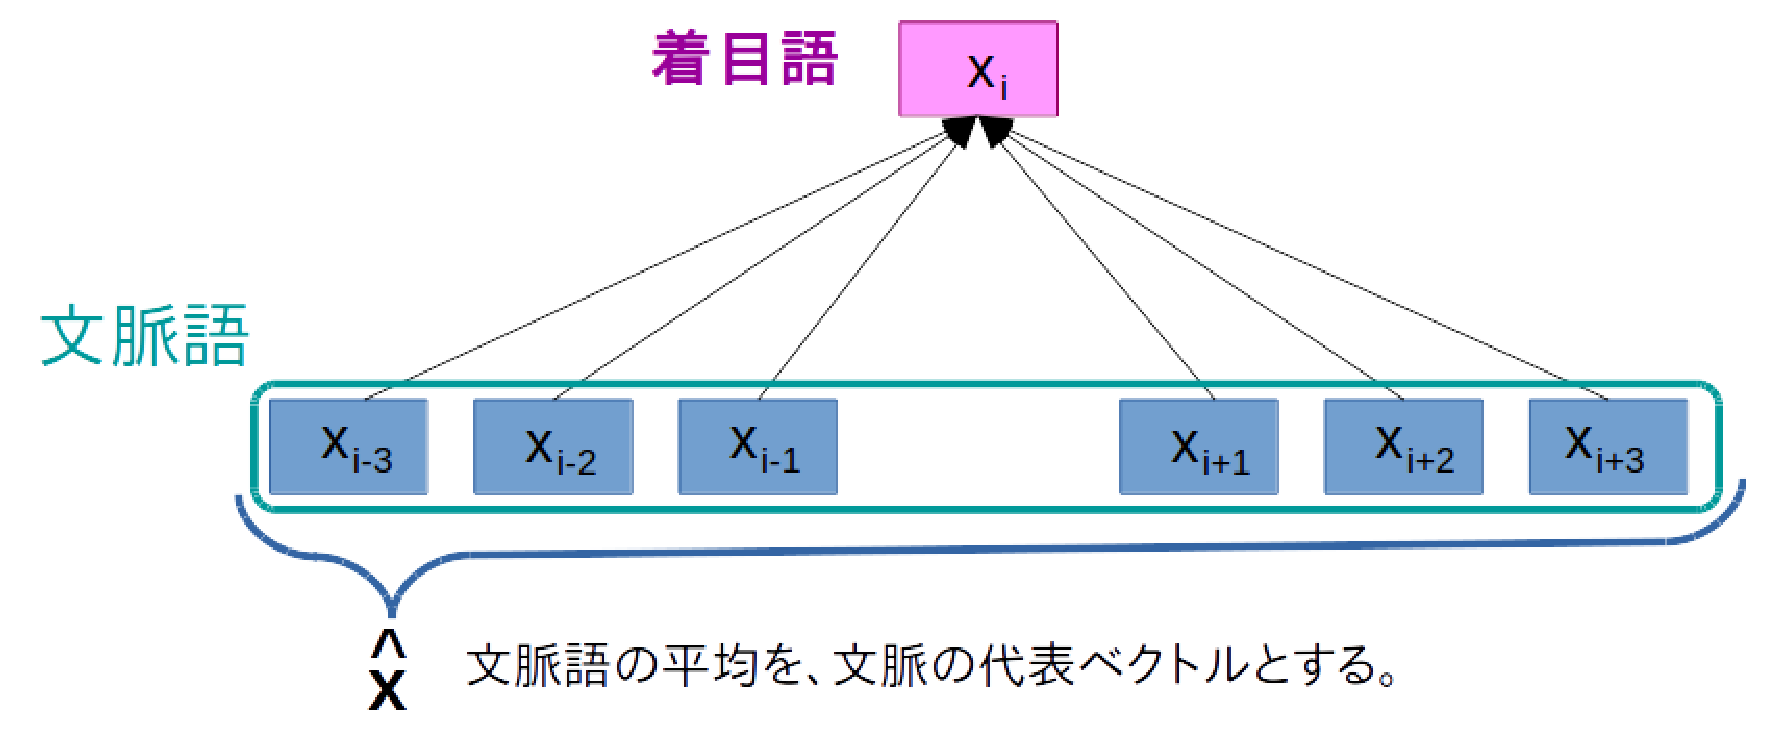
\includegraphics[width=12.5cm]{../images/CBoW.eps}
  \caption{CBoWによるベクトル構築イメージ}
\end{figure}

着目形態素の前後n(下図では3)個の形態素を文脈語とし、文脈語の表現ベクトルの平均を、着目形態素$x_i$の文脈を代表するベクトル$\widehat{x}$として、与えられた文脈中に、着目形態素$x_i$が出現する確率$p(x_i|\widehat{x})$は、
\begin{eqnarray}
  \label{cbow_p}
  p(x_i|\widehat{x}) = \frac{exp(\widehat{x}^Tx)}{\Sigma_{x'\in\nu}exp(\widehat{x}^Tx')}
\end{eqnarray}
と表せる。ここで$\nu$はコーパス中の全形態素からなる語彙集合であり、x'は$\nu$中の単語である。\\
文脈語の代表ベクトル算出時に語順を無視しているため、同じく語順を無視して文や文書ベクトルを導出する\textbf{Bag-of-Wordsモデル}の拡張とみなすことができる。

式(\ref{cbow_p})で導出できる確率を学習していく。学習過程については、次のモデルで学習する確率を説明した後に述べる。

\subsection{連続スキップグラムモデル}
\textbf{連続スキップグラムモデル}(continuous Skip-gram model, Sg model)では、連続単語袋詰モデルとは逆に、与えられた文脈語から着目形態素の出現を予測するものとなっている。
\begin{figure}[h]
  \centering
  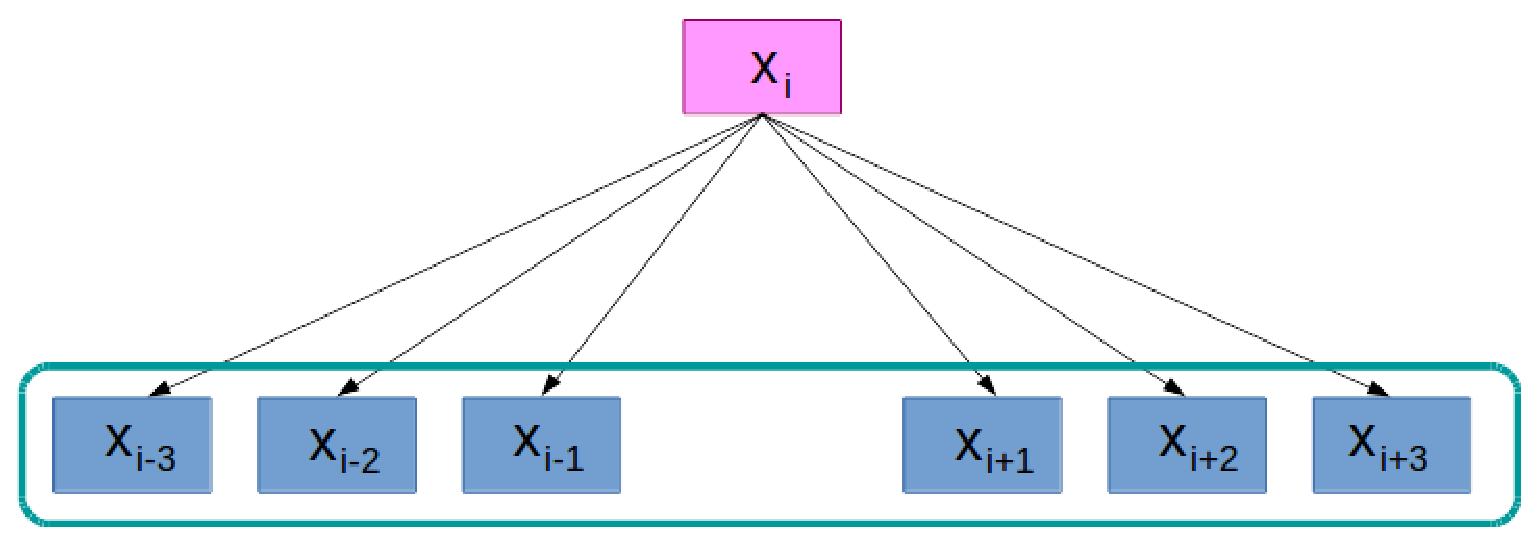
\includegraphics[width=12.5cm]{../images/Sg.eps}
  \caption{Sgによるベクトル構築イメージ}
\end{figure}

着目形態素$x_i$から文脈語を予測する場合の確率$p(x_{i-n},...,x_{i-1},x_{i+1},...,x_{i+n}|x_i)$は、着目形態素$x_i$が与えられた時、文脈語$x_{i-n},...,x_{i-1},x_{i+1},...,x_{i+n}$の出現確立がすべて独立であると仮定して、
\begin{eqnarray}
  \label{cskip_p}
  p(x_{i-n},...,x_{i-1},x_{i+1},...,x_{i+n}|x_i) = \frac{exp(x_i^TX)}{\Sigma_{X'\in\nu(x)}exp(x^TX')}
\end{eqnarray}
と表せる。ここで$\nu(x)$はコーパス中で着目形態素$x_i$と共起している文脈語の集合である。\\
文脈語の独立性を仮定することで、
\begin{eqnarray}
  p(x_{i-n},...,x_{i-1},x_{i+1},...,x_{i+n}|x_i) = p(x_{i-n}|x_i),...,p(x_{i-1}|x_i),p(x_{i+1}|x_i),...,p(x_{i+n}|x_i) \nonumber
\end{eqnarray}
と表すことができ、スキップグラムモデルでの確率計算を簡単にしている。

\subsection{二つの学習モデルの違い}
連続スキップグラムモデルでは、一つの着目形態素対、一つの文脈語の関係から確率計算を行うので、少ないコーパスからでも一定の精度のモデルを学習できることが期待できる。これに対し連続単語袋詰めモデルでは複数の文脈語から一つの着目形態素を予測するモデルであるため、複数の文脈語からなる単語列が、コーパス中に複数回出現している必要がある。したがって、連続スキップグラムモデルよりも大きなコーパスデータが必要となる。\cite{book_wm}

\section{モデルの最適化}
本節ではいよいよ、前節で導出した確率の最適化について述べていく。

まず、式(\ref{cbow_p}),(\ref{cskip_p})の右辺は\textbf{ソフトマックス関数}(softmax function)と呼ばれる関数の形になっており、このソフトマックス関数について述べる。

\subsection{ソフトマックス関数}
\textbf{ソフトマックス関数}(softmax function)は、N個の実数出力を、確率値に変換するのによく用いられる関数である。
\begin{eqnarray}
  \label{softmax_p}
  softmax(x_i) = \frac{exp(x_i)}{\Sigma_{j=1}^{N}exp(x_j)}
\end{eqnarray}
ソフトマックス関数が持つ特徴として、
\begin{itemize}
  \item 出力値が0から1の範囲内
  \item $\Sigma_{i=1}^Nsoftmax(x_i)=1$を満たす
\end{itemize}
というものがあり、これによって出力値を確率値として解釈可能にする。

\subsection{}

\subsection{負例サンプリング}

\subsection{階層型ソフトマックス}
